\documentclass[10pt]{article}

%---GEOMETRY

\usepackage{geometry}
   \geometry{verbose,tmargin=0.75in,bmargin=0.75in,%
     lmargin=0.7in,rmargin=0.4in,headheight=0.25in,%
     headsep=0.2in,footskip=0.4in}%

%---COMMENTS---
\usepackage{comment}

%---CODE OUTPUT---
\usepackage{listings}
\lstset
{ %Formatting for code in appendix
    language=Matlab,
    basicstyle=\footnotesize,
    numbers=left,
    stepnumber=1,
    showstringspaces=false,
    tabsize=4,
    breaklines=true,
    breakatwhitespace=false,
    escapeinside={(*}{*)}
}

\newcommand{\codeword}[1]{\texttt{#1}}

%---HYPERLINKS---

\RequirePackage{hyperref}
\hypersetup{
    colorlinks=true, %set true if you want colored links
    linktoc=all     %set to all if you want both sections and subsections linked
}

\begin{comment}
    citecolor=stycitecolor,
    filecolor=styfilecolor,
    linkcolor=stylinkcolor,
    urlcolor=styurlcolor
\end{comment}

%---MATHS PACKAGES---

\usepackage{math}

%---THEOREMS

\usepackage{altthms}

\theoremstyle{definition}

\renewtheorem{exercise}{Exercise}[section]
\renewcommand*{\theexercise}{\thesection-\arabic{exercise}}

%---INDEX---

\usepackage{imakeidx}
\makeindex

%---PLOTS---
\usepackage{graphicx}
\graphicspath{ {./images/} }

%---BIBLIOGRAPHY---

\usepackage[backend=biber, style=alphabetic]{biblatex}
\addbibresource{bibliography.bib}

%---ENUMERATION---

\usepackage{enumitem}

%---TITLE---

\title{CS285: Deep Reinforcement Learning \\ Assignment 2 \\ Written Report}
\author{Alan Sorani}
\date{\today}

\begin{document}

\maketitle

\section{Analysis}

\begin{enumerate}
\item
\begin{enumerate}[label=(\alph*)]
\item
Using policy gradients, we have
\begin{equation} \label{1-policy-gradients}
\nabla J\prs{\theta} = \mbb{E}_{\tau \sim p_\theta\prs{\tau}} \brs{\prs{\sum_{t = 1}^\infty \nabla_\theta \log \pi_\theta\prs{a_{i,t} \mid s_{i,t}}} R\prs{\tau}} \text{.}
\end{equation}

Due to the simplicity of our MDP, we can easily enumerate all the possible trajectories $\tau$ based on the first time-step $t$ for which $s_t = S_F$. Let $\tau_i$ be the trajectory for which $s_{i,j} = s_1$ for all $j < i$ and for which $s_{i,i} = s_F$ (and therefore $s_{i,j} = S_F$ for all $j > i$). The probablity of the trajectory $\tau_i$ under the policy $\pi_{\theta}$ is then $\theta^{i-1} \prs{1 - \theta}$. We see that $R\prs{\tau_i} = \sum_{j=1}^{i} r\prs{s_{i,j} \mid a_{i,j}} = \sum_{j=1}^{i-1} 1 = i-1$.

Writing the expectation of \eqref{1-policy-gradients} explicitly, we get
\begin{align*}
\nabla J\prs{\theta} &= \sum_{i=1}^{\infty} p_\theta\prs{\tau_i} \brs{\prs{\prs{\sum_{t = 1}^{i-1} \nabla_\theta \log\prs{\theta}} + \nabla_\theta \log\prs{1 - \theta}} \prs{i-1}}
\\&= \sum_{i=1}^{\infty} \theta^{i-1} \prs{1 - \theta} \brs{\prs{\frac{i-1}{\theta} - \frac{1}{1-\theta}} \prs{i-1}}
\\&= \sum_{i=1}^{\infty} \theta^{i-1} \brs{\prs{\frac{\prs{i-1}\prs{1 - \theta}}{\theta} - 1} \prs{i-1}}
\\&= \sum_{i=1}^{\infty} \theta^{i-1} \brs{\prs{\frac{\prs{i-1}\prs{1 - \theta} - \theta}{\theta}} \prs{i-1}}
\\&= \sum_{i=1}^{\infty} \theta^{i-2} \brs{\prs{i - \theta i - 1 + \theta - \theta}\prs{i-1}}
\\&= \sum_{i=1}^{\infty} \theta^{i-2} \prs{i-\theta i - 1}\prs{i-1}
\\&= \prs{1-\theta} \sum_{i=1}^{\infty} i \prs{i-1} \theta^{i-2} - \sum_{i=1}^{\infty} \prs{i-1} \theta^{i-2} \text{.}
\end{align*}
Finally, we have
\begin{align*}
\prs{1 - \theta} \sum_{i=1}^{\infty} i \prs{i-1} \theta^{i-2} &=
\prs{1 - \theta} \sum_{i=1}^{\infty} \frac{\diff^2}{\diff^2 \theta} \theta^i
\\&=
\prs{1 - \theta} \frac{\diff^2}{\diff^2 \theta} \sum_{i=1}^{\infty} \theta^i
\\&=
\prs{1 - \theta} \frac{\diff^2}{\diff^2 \theta} \frac{\theta}{1 - \theta}
\\&=
\prs{1 - \theta} \frac{\diff}{\diff \theta} \frac{1}{\prs{1 - \theta}^2}
\\&= \prs{1 - \theta} \cdot \prs{- \frac{2}{\prs{1-\theta}^3}}
\\&= \frac{2}{\prs{1-\theta}^2}
\end{align*}
and
\begin{align*}
\sum_{i=1}^{\infty} \prs{i-1} \theta^{i-2}
&=
\sum_{i=1}^{\infty} \frac{\diff}{\diff \theta} \theta^{i-1}
\\&=
\frac{\diff}{\diff \theta} \sum_{i=1}^{\infty} \theta^{i-1}
\\&=
\frac{\diff}{\diff \theta} \frac{1}{1 - \theta}
\\&= \frac{1}{\prs{1-\theta}^2} \text{,}
\end{align*}
so we get
\begin{align*}
\nabla J\prs{\theta}
&=
\frac{2}{\prs{1-\theta}^2} - \frac{1}{\prs{1-\theta}^2} = \frac{1}{\prs{1 - \theta}^2} \text{.}
\end{align*}

\item We shall now compute $\mbb{E}_{\tau \sim \pi_\theta}\brs{R\prs{\tau}}$ directly and verify that \[\nabla \mbb{E}_{\tau \sim \pi_\theta}\brs{R\prs{\tau}} = \frac{1}{\prs{1 - \theta}^2} \text{.}\]
We have
\begin{align*}
\mbb{E}_{\tau \sim \pi_\theta}\brs{R\prs{\tau}} &= \sum_{i = 1}^{\infty} p_{\theta}\prs{\tau_i} R\prs{\tau_i}
\\&=
\sum_{i=1}^{\infty} \theta^{i-1} \prs{1 - \theta} \prs{i-1}
\\&=
\prs{1 - \theta} \sum_{i = 1}^{\infty} \theta^{i-1} \prs{i-1}
\\&=
\prs{1 - \theta} \sum_{i=1}^{\infty} \frac{\diff}{\diff \theta} \theta^i
\\&=
\prs{1 - \theta} \frac{\diff}{\diff \theta} \sum_{i=1}^{\infty} \theta^i
\\&=
\prs{1 - \theta} \frac{\diff}{\diff \theta} \frac{\theta}{1 - \theta}
\\&=
\prs{1 - \theta} \cdot \frac{1}{\prs{1 - \theta}^2}
\\&= \frac{1}{1 - \theta}
\end{align*}
and then indeed
\begin{align*}
\nabla \mbb{E}_{\tau \sim \pi_\theta}\brs{R\prs{\tau}} &= \nabla \frac{1}{1 - \theta} = \frac{1}{\prs{1 - \theta}^2} \text{.}
\end{align*}
\end{enumerate}

\item
We have
\begin{align*}
\Var\brs{X} = \mbb{E}\brs{X^2} - \mbb{E}\brs{X}^2 \text{,}
\end{align*}
so
\begin{align*}
\Var_{\tau \sim p_\theta\prs{\tau}}\brs{\nabla_\theta \log p_\theta\prs{\tau} r\prs{\tau}} &=
\mbb{E}_{\tau \sim p_\theta\prs{\tau}}\brs{\prs{\nabla_\theta \log p_\theta\prs{\tau} r\prs{\tau}}^2}
- \mbb{E}_{\tau \sim p_\theta\prs{\tau}}\brs{\nabla_\theta \log p_\theta\prs{\tau} r\prs{\tau}}^2
\\&=
\mbb{E}_{\tau \sim p_\theta\prs{\tau}}\brs{\prs{\nabla_\theta \log p_\theta\prs{\tau} r\prs{\tau}}^2}
- \nabla J\prs{\theta}^2
\\&=
\mbb{E}_{\tau \sim p_\theta\prs{\tau}}\brs{\prs{\nabla_\theta \log p_\theta\prs{\tau} r\prs{\tau}}^2} - \frac{1}{\prs{1 - \theta}^4} \text{.}
\end{align*}
Now, using our computations from the previous part, we get
\begin{align*}
\mbb{E}_{\tau \sim p_\theta\prs{\tau}}\brs{\prs{\nabla_\theta \log p_\theta\prs{\tau} r\prs{\tau}}^2} &=
\sum_{i=1}^{\infty} p_\theta\prs{\tau_i} \brs{\prs{\prs{\sum_{t = 1}^{i-1} \nabla_\theta \log\prs{\theta}} + \nabla_\theta \log\prs{1 - \theta}} \prs{i-1}}^2
\\&=
\sum_{i=1}^{\infty} \theta^{i-1} \prs{1 - \theta} \brs{\prs{\frac{i - 1}{\theta} - \frac{1}{1 - \theta}} \prs{i-1}}^2
\\&=
\sum_{i=1}^{\infty} \frac{\theta^{i-3}}{1 - \theta} \prs{i \prs{1 - \theta} - 1}^2 \prs{i-1}^2
\\&=
\frac{1}{1 - \theta} \sum_{i=1}^{\infty} \theta^{i-3} \prs{i \prs{1 - \theta} - 1}^2 \prs{i-1}^2
\\&=
\frac{1}{1 - \theta} \sum_{i=1}^{\infty} \theta^{i-3} \prs{i^2 \prs{1-\theta}^2 - 2i\prs{1-\theta} + 1} \prs{i^2 -2i + 1}
\\&= 
\frac{1}{\theta^3\prs{1 - \theta}} \sum_{i=1}^{\infty} \theta^i \prs{i^4 \theta^2 -2i^4 \theta +i^4 - 2i^3 \theta^2 + 6i^3 \theta -4i^3 +i^2 \theta^2 - 6i^2 \theta +6 i^2 + 2i\theta -4i + 1} \text{.}
\end{align*}
We get that
\begin{align*}
\mbb{E}_{\tau \sim p_\theta\prs{\tau}}\brs{\prs{\nabla_\theta \log p_\theta\prs{\tau} r\prs{\tau}}^2} &= \frac{1}{\theta^3\prs{1 - \theta}} \prs{S_1 - S_2 + S_3 - S_4 + S_5 - S_6 + S_7 - S_8 + S_9 + S_10 - S_11 + S_12}
\end{align*}
where
\begin{align*}
S_1 &= \sum_{i=1}^{\infty} i^4 \theta^{i+2}, & & & S_7 &= \sum_{i=1}^{\infty} i^2 \theta^{i+2}
\\ 
S_2 &= 2 \sum_{i=1}^{\infty} i^4 \theta^{i+1}, & & &  S_8 &= 6 \sum_{i=1}^{\infty} i^2 \theta^{i+1}
\\
S_3 &= \sum_{i=1}^{\infty} i^4 \theta^i, & & &  S_9 &= 6 \sum_{i=1}^{\infty} i^2 \theta^i
\\
S_4 &= 2 \sum_{i=1}^{\infty} i^3 \theta^{i+2}, & & &  S_{10} &= 2 \sum_{i=1}^{\infty} i \theta^{i+1}
\\
S_5 &= 6 \sum_{i=1}^{\infty} i^3 \theta^{i+1}, & & &  S_{11} &= 4 \sum_{i=1}^{\infty} i \theta^i
\\
S_6 &= 4 \sum_{i=1}^{\infty} i^3 \theta^i, & & &  S_{12} &= \sum_{i=1}^{\infty} \theta^i \text{.}
\end{align*}
Now,
\begin{align*}
\sum_{i = 1}^{\infty} \theta^i &= \frac{\theta}{1 - \theta}
\end{align*}
so by differentiating
\begin{align*}
\sum_{i=1}^{\infty} i \theta^{i-1} &= \frac{1}{\prs{1 - \theta}^2}
\end{align*}
and by multiplying by $\theta$
\begin{align*}
\sum_{i=1}^{\infty} i \theta^i &= \frac{\theta}{\prs{1 - \theta}^2} \text{.}
\end{align*}
By differentiating this and then multiplying by $\theta$ we get
\begin{align*}
\sum_{i=1}^{\infty} i^2 \theta^i = \frac{\theta^2 + \theta}{\prs{1-\theta}^3} \text{.}
\end{align*}
By repeating this we get
\begin{align*}
\sum_{i=1}^{\infty} i^3 \theta^i = \frac{\theta^3 + 4\theta^2 + \theta}{\prs{1-\theta}^4}
\end{align*}
and finally
\begin{align*}
\sum_{i=1}^{\infty} i^4 \theta^i = \frac{\theta^4 + 11 \theta^3 + 11\theta^2 + \theta}{\prs{1-\theta}^5} \text{.}
\end{align*}
Using these equations we get
\begin{align*}
S_1 &= \theta^2 \cdot \frac{\theta^4 + 11 \theta^3 + 11\theta^2 + \theta}{\prs{1-\theta}^5}, & & & S_7 &= \theta^2 \cdot \frac{\theta^2 + \theta}{\prs{1-\theta}^3}
\\ 
S_2 &= 2 \theta \cdot \frac{\theta^4 + 11 \theta^3 + 11\theta^2 + \theta}{\prs{1-\theta}^5}, & & &  S_8 &= 6 \theta \cdot \frac{\theta^2 + \theta}{\prs{1-\theta}^3}
\\
S_3 &= \frac{\theta^4 + 11 \theta^3 + 11\theta^2 + \theta}{\prs{1-\theta}^5}, & & &  S_9 &= 6 \cdot \frac{\theta^2 + \theta}{\prs{1-\theta}^3}
\\
S_4 &= 2 \theta^2 \cdot \frac{\theta^3 + 4\theta^2 + \theta}{\prs{1-\theta}^4}, & & &  S_{10} &= 2 \theta \cdot \frac{\theta}{\prs{1 - \theta}^2}
\\
S_5 &= 6 \theta \cdot \frac{\theta^3 + 4\theta^2 + \theta}{\prs{1-\theta}^4}, & & &  S_{11} &= 4 \cdot \frac{\theta}{\prs{1 - \theta}^2}
\\
S_6 &= 4 \cdot \frac{\theta^3 + 4\theta^2 + \theta}{\prs{1-\theta}^4}, & & &  S_{12} &= \frac{\theta}{1 - \theta} \text{.}
\end{align*}
Going back to the calculation of $\mbb{E}_{\tau \sim p_\theta\prs{\tau}}\brs{\prs{\nabla_\theta \log p_\theta\prs{\tau} r\prs{\tau}}^2}$ we get
\begin{align*}
\mbb{E}_{\tau \sim p_\theta\prs{\tau}}\brs{\prs{\nabla_\theta \log p_\theta\prs{\tau} r\prs{\tau}}^2}
&=
\frac{1}{\theta^3\prs{1 - \theta}} \prs{S_1 - S_2 + S_3 - S_4 + S_5 - S_6 + S_7 - S_8 + S_9 + S_10 - S_11 + S_12}
\\&=
\frac{1}{\theta^3\prs{1 - \theta}} \cdot \frac{\theta^2 \prs{4 \theta^2 + 9\theta + 1}}{\prs{1-\theta}^3}
\\&=
\frac{4 \theta^2 + 9\theta + 1}{\theta \prs{1-\theta}^4}
\end{align*}
and so
\begin{align*}
\Var_{\tau \sim p_\theta\prs{\tau}}\brs{\nabla_\theta \log p_\theta\prs{\tau} r\prs{\tau}}
&=
\frac{4 \theta^2 + 9\theta + 1}{\theta \prs{1-\theta}^4} - \frac{1}{\prs{1-\theta}^4}
\\&=
\frac{4 \theta^2 + 8\theta + 1}{\theta \prs{1-\theta}^4} \text{.}
\end{align*}
To find the values of $\theta$ which minimize or maximize the variance, we compare
\[\frac{\diff}{\diff \theta} \Var_{\tau \sim p_\theta\prs{\tau}}\brs{\nabla_\theta \log p_\theta\prs{\tau} r\prs{\tau}} = \frac{12\theta^3 + 36\theta^2 + 5\theta - 1}{\theta^2 \prs{1-\theta}^5}\]
to $0$. We get that the variance is minimal for $\theta \approx 0.10988$ and goes to infinity as $\theta$ approaches $0$ or $1$.

\item
\begin{enumerate}[label=(\alph*)]
\item
An advantage estimator is a function $A$, possibly dependent on time, which gives the following estimate:
\begin{align*}
\nabla J\prs{\theta} \approx \mbb{E}_{\tau \sim p_\theta\prs{\tau}}\brs{\sum_{t=1}^{\infty} \nabla_{\theta} \log \pi_\theta \prs{a_{i,t} \mid s_{i,t}} A_t\prs{\tau}} \text{.}
\end{align*}
We consider \[A_t\prs{\tau} = \sum_{t' = t}^{\infty} r\prs{s_{i,t'}, a_{i,t'}}\]
which is the \emph{return-to-go} advantage estimator.

We see that for any $t \in \mbb{N}_+$,
\begin{align*}
A_t\prs{\tau_i} &= \sum_{t'=t}^i r\prs{s_{i,t'} \mid a_{i,t'}} = \sum_{t' = t}^{i-1} 1 = i-1-\prs{t-1} = i-t \text{.}
\end{align*}
Hence
\begin{align*}
\mbb{E}_{\tau \sim p_\theta\prs{\tau}}\brs{\sum_{t=1}^{\infty} \nabla_{\theta} \log \pi_\theta \prs{a_{i,t} \mid s_{i,t}} A_t\prs{\tau}} &=
\sum_{i=1}^{\infty} p_\theta\prs{\tau_i} \brs{\sum_{t = 1}^{i-1} \nabla_\theta \log\prs{\theta} \cdot \prs{i-t}}
\\&=
\sum_{i=1}^{\infty} \theta^{i-1} \prs{1-\theta} \prs{\sum_{t=1}^{i-1} \frac{i-t}{\theta}}
\\&=
\sum_{i=1}^{\infty} \theta^{i-2} \prs{1-\theta} \prs{i\prs{i-1} - \sum_{t=1}^{i-1} t}
\\&=
\sum_{i=1}^{\infty} \theta^{i-2} \prs{1-\theta} \prs{i\prs{i-1} - \frac{i\prs{i-1}}{2}}
\\&=
\frac{1}{2} \sum_{i=1}^{\infty} \theta^{i-2} \prs{1-\theta} i \prs{i-1} \\&=
\frac{1}{2} \prs{\sum_{i=1}^{\infty} \theta^{i-2} i^2 - \sum_{i=1}^{\infty} \theta^{i-2} i - \sum_{i=1}^{\infty} \theta^{i-1} i^2 + \sum_{i=1}^{\infty} \theta^{i-1} i} \text{.}
\end{align*}
Write
\begin{align*}
S'_1 &\coloneqq \sum_{i=1}^{\infty} \theta^{i-2} i^2 \\
S'_2 &\coloneqq \sum_{i=1}^{\infty} \theta^{i-2} i \\
S'_3 &\coloneqq \sum_{i=1}^{\infty} \theta^{i-1} i^2 \\
S'_4 &\coloneqq \sum_{i=1}^{\infty} \theta^{i-1} i \text{.}
\end{align*}
We calculated in the previous part that
\begin{align*}
S'_4 = \frac{1}{\prs{1-\theta}^2} \text{.}
\end{align*}
Then
\begin{align*}
S'_2 = \sum_{i=1}^{\infty} \theta^{i-2} i = \theta^{-1} \sum_{i=1}^{\infty} \theta^{i-1} i = \theta^{-1} S'_4 = \frac{1}{\theta \prs{1-\theta}^2} \text{.} 
\end{align*}
We also showed that
\begin{align*}
\sum_{i=1}^\infty i^2 \theta^i = \frac{\theta^2 + \theta}{\prs{1-\theta}^3} \text{,}
\end{align*}
so similarly we get
\begin{align*}
S'_3 = \frac{\theta + 1}{\prs{1-\theta}^3}
\end{align*}
and
\begin{align*}
S'_1 = \frac{\theta + 1}{\theta \prs{1-\theta}^3} \text{.}
\end{align*}
Finally, we get
\begin{align*}
\mbb{E}_{\tau \sim p_\theta\prs{\tau}}\brs{\sum_{t=1}^{\infty} \nabla_{\theta} \log \pi_\theta \prs{a_{i,t} \mid s_{i,t}}}
&=
\frac{1}{2} \prs{S'_1 - S'_2 - S'_3 + S'_4}
\\&=
\frac{1}{2} \cdot \frac{\prs{\theta+1} - \prs{1-\theta} - \prs{\theta^2 + \theta} + \theta\prs{1-\theta}}{\theta \prs{1-\theta}^3}
\frac{1}{2} \cdot \frac{-2 \theta^2 + 2\theta}{\theta \prs{1-\theta}^3}
\\&=
\frac{\theta\prs{1-\theta}}{\theta \prs{1-\theta}^3}
\\&=
\frac{1}{\prs{1-\theta}^2}
\\&=
\nabla J\prs{\theta} \text{.}
\end{align*}
Hence our advantage estimator is unbiased in the sense that in expectation it has the same value
\[\mbb{E}_{\tau \sim p_\theta\prs{\tau}}\brs{\sum_{t=1}^{\infty} \nabla_{\theta} \log \pi_\theta \prs{a_{i,t} \mid s_{i,t}} A_t\prs{\tau}}\]
as the true value of the gradient, $\nabla J\prs{\theta}$.

\item
We now compute the variance of the return-to-go policy variant. From what we've learnt in the lecture, return-to-go is used to reduce variance, so we expect a lower variance than the one we got in part 2.

We have
\begin{align*}
\Var_{\tau \sim p_\theta\prs{\tau}}\brs{\sum_{t=1}^{\infty} \nabla_{\theta} \log \pi_\theta \prs{a_{i,t} \mid s_{i,t}} A_t\prs{\tau}}
&=
\mbb{E}_{\tau \sim p_\theta\prs{\tau}}\brs{\prs{\sum_{t=1}^{\infty} \nabla_{\theta} \log \pi_\theta \prs{a_{i,t} \mid s_{i,t}} A_t\prs{\tau}}^2}
\\&-
\mbb{E}_{\tau \sim p_\theta\prs{\tau}}\brs{\sum_{t=1}^{\infty} \nabla_{\theta} \log \pi_\theta \prs{a_{i,t} \mid s_{i,t}} A_t\prs{\tau}}^2
\\&= \mbb{E}_{\tau \sim p_\theta\prs{\tau}}\brs{\prs{\sum_{t=1}^{\infty} \nabla_{\theta} \log \pi_\theta \prs{a_{i,t} \mid s_{i,t}} A_t\prs{\tau}}^2} - \frac{1}{\prs{1-\theta}^4} \text{.}
\end{align*}

Now, using our computations from part 3(a) we get
\begin{align*}
\mbb{E}_{\tau \sim p_\theta\prs{\tau}}\brs{\prs{\sum_{t=1}^{\infty} \nabla_{\theta} \log \pi_\theta \prs{a_{i,t} \mid s_{i,t}} A_t\prs{\tau}}^2} &= \sum_{i=1}^{\infty} p_\theta\prs{\tau_i} \prs{\sum_{t=1}^{i-1} \nabla_\theta \log\prs{\theta} \cdot \prs{i-t}}^2
\\&=
\frac{1}{4} \sum_{i=1}^{\infty} \theta^{i-3} \prs{1-\theta} i^2 \prs{i-1}^2
\\&=
\frac{1 - \theta}{4 \theta^3} \sum_{i=1}^\infty \theta^i i^2 \prs{i^2 -2i + 1}
\\&=
\frac{1 - \theta}{4 \theta^3} \sum_{i=1}^\infty \theta^i \prs{i^4 -2i^3 + i^2}
\\&=
\frac{1 - \theta}{4 \theta^3} \prs{\sum_{i=1}^{\infty} \theta^i i^4 -2 \sum_{i=1}^{\infty} \theta^i i^3 + \sum_{i=1}^\infty \theta^i i^2}
\\&=
\frac{1 - \theta}{4 \theta^3} \prs{\frac{\theta^4 + 11 \theta^3 + 11 \theta^2 + \theta}{\prs{1-\theta}^5} - 2 \cdot \frac{\theta^3 + 4\theta^2 + \theta}{\prs{1-\theta}^4} + \frac{\theta^2 + \theta}{\prs{1-\theta}^3}}
\\&=
\frac{1 - \theta}{4 \theta^3} \cdot \frac{4 \theta^2 \prs{\theta^2 + 4\theta + 1}}{\prs{1 - \theta}^5}
\\&=
\frac{\theta^2 + 4 \theta + 1}{\theta \prs{1-\theta}^4}
\end{align*}
where the second-to-last equation is from calculations in part 2.
Hence
\begin{align*}
\Var_{\tau \sim p_\theta\prs{\tau}}\brs{\sum_{t=1}^{\infty} \nabla_{\theta} \log \pi_\theta \prs{a_{i,t} \mid s_{i,t}} A_t\prs{\tau}} &=
\frac{\theta^2 + 4\theta + 1}{\theta \prs{1-\theta}^4} - \frac{1}{\prs{1-\theta}^4} = \frac{\theta^2 + 3\theta + 1}{\theta \prs{1-\theta}^4} \text{.}
\end{align*}
In \Cref{fig:variance} we plot the variance before and after using return-to-go, and in \Cref{fig:variance-diff} we plot the reduction in variance gained by using return-to-go, which we notice is non-negative for all $\theta$.

\begin{figure}[h]
\caption{The variance, depending on $\theta$, of the policy gradient without return-to-go (in blue) and with return to go (in orange).}
\label{fig:variance}
\centering
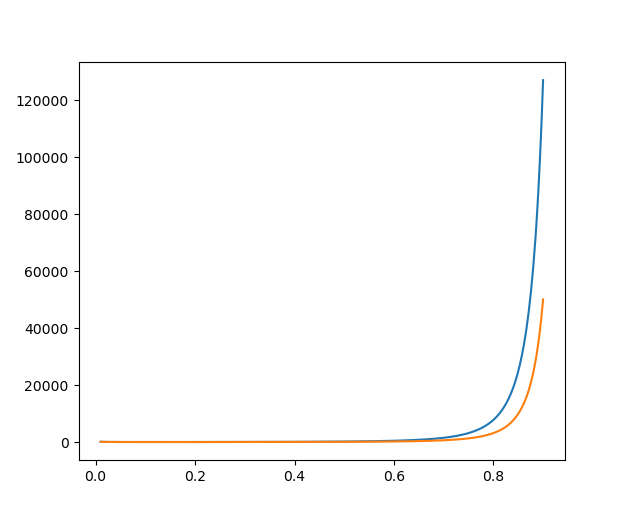
\includegraphics[width=8cm]{Figure_1}
\end{figure}

\begin{figure}[h]
\caption{The reduction in variance gained by using return-to-go, as a function of $\theta$.}
\label{fig:variance-diff}
\centering
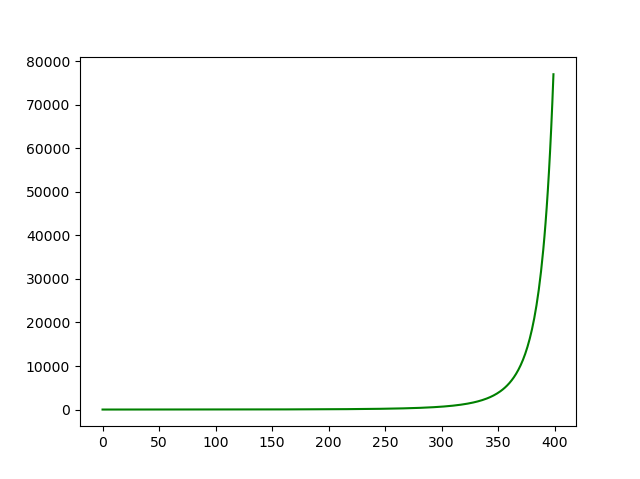
\includegraphics[width=8cm]{Figure_2}
\end{figure}

\end{enumerate}

\item
\begin{enumerate}[label=(\alph*)]
\item
We have
\begin{align*}
\nabla_\theta J\prs{\theta} = \mbb{E}_{\tau \sim p_{\theta'}\prs{\tau}}\brs{\frac{\prod_{t=1}^H \pi_\theta\prs{a_t \mid s_t}}{\prod_{t=1}^H\pi_{\theta'}\prs{a_t \mid s_t}} \nabla_\theta \log p_\theta\prs{\tau} R\prs{\tau}} \text{.}
\end{align*}
Let $\tau_0 = \prs{s_1, \ldots, s_H}$. Because $R = \chi_{\tau_0}$, we get
\begin{align*}
\nabla_\theta J\prs{\theta} &= p_{\theta'}\prs{\tau_0} \frac{p_{\theta}\prs{\tau_0}}{p_{\theta'}\prs{\tau_0}} \nabla_\theta \log p_\theta\prs{\tau_0}
\\&=
p_\theta\prs{\tau_0} \nabla_\theta \log p_\theta\prs{\tau_0}
\\&=
\nabla_\theta p_\theta\prs{\tau_0}
\\&=
\nabla_\theta \prod_{t=1}^{H-1} p_\theta\prs{a_1 \mid s_t} \text{.}
\end{align*}
\item
We have
\begin{align*}
\Var_{\tau \sim p_{\theta'}\prs{\tau}}\brs{\frac{\prod_{t=1}^H \pi_\theta\prs{a_t \mid s_t}}{\prod_{t=1}^H\pi_{\theta'}\prs{a_t \mid s_t}} \nabla_\theta \log p_\theta\prs{\tau} R\prs{\tau}}
&=
\mbb{E}_{\tau \sim p_{\theta'}\prs{\tau}}\brs{\prs{\frac{\prod_{t=1}^H \pi_\theta\prs{a_t \mid s_t}}{\prod_{t=1}^H\pi_{\theta'}\prs{a_t \mid s_t}} \nabla_\theta \log p_\theta\prs{\tau} R\prs{\tau}}^2}
\\&
-\mbb{E}_{\tau \sim p_{\theta'}\prs{\tau}}\brs{\frac{\prod_{t=1}^H \pi_\theta\prs{a_t \mid s_t}}{\prod_{t=1}^H\pi_{\theta'}\prs{a_t \mid s_t}} \nabla_\theta \log p_\theta\prs{\tau} R\prs{\tau}}^2
\\&=
p_{\theta'} \prs{\frac{p_\theta\prs{\tau_0}}{p_{\theta'}\prs{\tau_0}} \nabla_\theta \log p_\theta\prs{\tau_0}}^2 - \prs{\nabla_\theta \prod_{t=1}^{H-1} p_\theta\prs{a_1 \mid s_t}}^2
\\&=
\frac{p_\theta\prs{\tau_0}^2}{p_{\theta'}\prs{\tau_0}} \prs{\nabla_\theta \log p_\theta\prs{\tau_0}}^2 - \prs{\nabla_\theta \prod_{t=1}^{H-1} p_\theta\prs{a_1 \mid s_t}}^2
\end{align*}
\end{enumerate}
Now, $p_\theta\prs{\tau_0}$ grows exponentially in $H$ and therefore so does its derivative. Then $\log p_\theta$ is a linear term in $H$ so its derivative is constant. We get that both of the summands approach zero, as the base of the exponent is smaller than $1$, and so the variance goes to $0$ as $H \rightarrow \infty$.
\end{enumerate}

\printbibliography
\printindex

\end{document}
